%%%%%%%%%%%%%%%%%%%%%%%%%%%%%%%%%%%%%%%%%
% By Mohammad Zandsalimy
%%%%%%%%%%%%%%%%%%%%%%%%%%%%%%%%%%%%%%%%%

\documentclass{article}

\usepackage{graphicx}
\usepackage{natbib}
\usepackage{amsmath}
\usepackage{mathtools}
\usepackage{pgfplots}
\usetikzlibrary{patterns}
\usepackage{adjustbox}
\usepackage{placeins}
\usepackage{multirow}
\usepackage{subcaption}
\usepackage{listings}
\usepackage{float}
\usepackage{hyperref}
\graphicspath{{./figures/}}
\renewcommand{\labelenumi}{\alph{enumi}.}

\title{Compressible Flow}
\author{Mohammad \textsc{Zandsalimy}}
\date{\today}


\begin{document}
\maketitle

% \begin{abstract}
% Text
% \end{abstract}

The inviscid compressible 1-dimensional flow is analyzed numerically using the finite volume method in the present project. The problem in question is the famous shock tube which is simulated from an initial condition to $t=0.15$ seconds. The initial conditions of this problem are presented in figure \ref{fig_initial_condition_1}. The domain length is 1 unit which is long enough so that no flow feature would reach either of the ends of the tube. The Euler equations are the governing equations of this problem. Two flux vector splitting schemes of Steger-Warming \cite{steger1981flux} and Roe \cite{van1987comparison} are utilized for this purpose. Time integration is fully explicit (implicit methods are readily applicable as well) including Explicit Euler and several Runge-Kutta methods. To prevent overshoots in the solution, several flux limiters are introduced, including, Superbee \cite{arora1997well}, Van Leer \cite{sweby1984high}, and 2nd order upwind limiters.

\begin{figure}[ht]
  \centering
  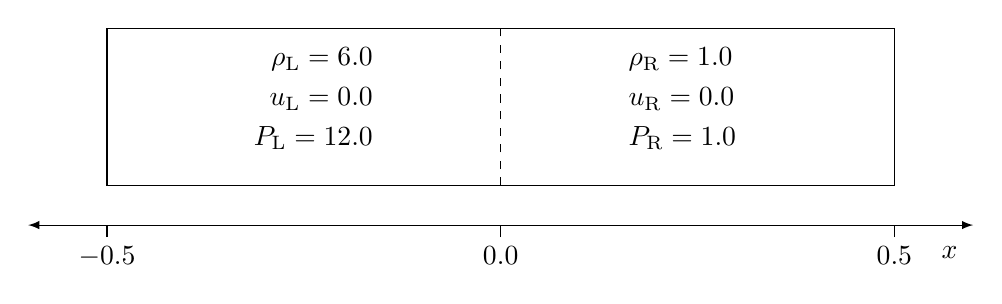
\begin{tikzpicture}
  \draw[black] (-5,0.5) rectangle (5,2.5);
  \draw[black, dashed] (0,0.5) -- (0,2.5);
  \draw[latex-latex, black] (-6,0) --  (6,0);
  \node[below] at (5,-0.1522) {$0.5$};
  \draw[black] (5,-0.1522) -- (5,0);
  \node[below] at (0,-0.1522) {$0.0$};
  \draw[black] (0,-0.1522) -- (0,0);
  \node[below] at (-5,-0.1522) {$-0.5$};
  \draw[black] (-5,-0.1522) -- (-5,0);
  \node[below] at (5.7,-.1522) {$x$};
  \node[right] at (1.5,2.1) {$\rho_{\text{R}}=1.0$};
  \node[right] at (1.5,1.6) {$u_{\text{R}}=0.0$};
  \node[right] at (1.5,1.1) {$P_{\text{R}}=1.0$};
  \node[left] at (-1.5,2.1) {$\rho_{\text{L}}=6.0$};
  \node[left] at (-1.5,1.6) {$u_{\text{L}}=0.0$};
  \node[left] at (-1.5,1.1) {$P_{\text{L}}=12.0$};
  \end{tikzpicture}
  \caption{The physical domain and initial conditions of the problem}
  \label{fig_initial_condition_1}
\end{figure}

The system of governing equations are presented in matrix form as follows,
\begin{equation}
\label{eq_main_1}
\dfrac{\partial U}{\partial t}+\dfrac{\partial F}{\partial x}=0
\end{equation}
in which the solution vector $U$ and flux $F$ are,
\begin{equation*}
U=
\left[
\begin{matrix}
\rho \\[10pt]
\rho u \\[10pt]
E \\
\end{matrix}
\right], \quad \quad
F=
\left[
\begin{matrix}
\rho u \\[10pt]
\rho u^2+ P\\[10pt]
u(E+P) \\
\end{matrix}
\right]
\end{equation*}
In these equations, $\rho$ is the fluid density, $u$ is velocity, $P$ is thermodynamic pressure, and $E$ is the total energy.
\begin{equation*}
E=\dfrac{P}{\gamma-1}+\dfrac{\rho u^2}{2}
\end{equation*}
Integrate equation \ref{eq_main_1} over a control volume with area $A=w \Delta x$ ($w$ is the channel width and $\Delta x$ is cell size in $x$ direction) and find the averaged equation.
\begin{equation*}
\dfrac{1}{A} \iint_{\Omega}\left[ \dfrac{\partial U}{\partial t}+\dfrac{\partial F}{\partial x} \right] dA=0
\end{equation*}
\begin{equation*}
\dfrac{1}{A} \iint_{\Omega}\left[ \dfrac{\partial U}{\partial t} \right] dA + \dfrac{1}{A} \iint_{\Omega}\left[\dfrac{\partial F}{\partial x} \right] dA=0
\end{equation*}
Use the Green's integral theorem for the flux ($\dfrac{\partial F}{\partial x}$) term,
\begin{equation*}
\dfrac{\partial }{\partial t} \left[ \dfrac{1}{A} \iint_{\Omega} U dA \right] + \dfrac{1}{A} \int_{\partial \Omega} F\cdot \vec{n} ds=0
\end{equation*}
\begin{equation*}
\dfrac{\partial \overline{U}_i}{\partial t} + \dfrac{1}{w \Delta x} \left[wF_{i+\frac{1}{2}}-wF_{i-\frac{1}{2}}+\Delta x\times 0-\Delta x\times 0\right]=0
\end{equation*}
\begin{equation}
\boxed{
\label{eq_main_2}
\dfrac{\partial \overline{U}_i}{\partial t} + \dfrac{F_{i+\frac{1}{2}}-F_{i-\frac{1}{2}}}{\Delta x}=0
}
\end{equation}

We can solve equation \ref{eq_main_2} using an explicit or implicit method. For this project we will opt for explicit methods. Rewrite the equation with explicit time advance,
\begin{equation}
\label{eq_main_3}
\delta \overline{U}_i =\overline{U}_i^{n+1}-\overline{U}_i^{n}=- \dfrac{\Delta t}{\Delta x} \left[F_{i+\frac{1}{2}}^{n}-F_{i-\frac{1}{2}}^{n} \right]
\end{equation}
Now, everything that is left is to calculate the fluxes on left and right faces of each cell, $F_{i+\frac{1}{2}}^{n}$ and  $F_{i-\frac{1}{2}}^{n}$. Drop the time level indicator, $n$, for convenience.

\section{Steger-Warming Flux Vector Splitting}
Steger and Warming proposed splitting the flux vector into two right and left moving components. Use characteristic theory for the splitting process. The flux vector can be written as follows,
\begin{equation*}
F=\dfrac{\partial F}{\partial U} U = AU
\end{equation*}
in which $A$ is,
\begin{equation*}
A=
\left[
\begin{matrix}
0 & 1 & 0 \\[10pt]
-\dfrac{u^2 (3-\gamma)}{2} & u(3-\gamma)& \gamma-1\\[10pt]
-\dfrac{\gamma u E}{\rho} +(\gamma-1) u^3 & \dfrac{\gamma E}{\rho}-\dfrac{3(\gamma-1) u^2}{2} & \gamma u\\
\end{matrix}
\right]
\end{equation*}
The goal is to split $A$ into two parts of right moving $A^+$ and left moving $A^-$ components and write,
\begin{equation}
\label{eq_flux_split_steger_1}
F_{i+\frac{1}{2}} = F_{i+\frac{1}{2}}^+ +F_{i+\frac{1}{2}}^- = \left(A^+ U\right)_{{i+\frac{1}{2}},i}+\left(A^- U\right)_{{i+\frac{1}{2}},i+1}
\end{equation}
In this equation, $\left(A^+ U\right)_{{i+\frac{1}{2}},i}$ is calculated from reconstructed solution variables on the right face of cell $i$ and $\left(A^- U\right)_{{i+\frac{1}{2}},i+1}$ is calculated from reconstructed solution variables on the left face of cell $i+1$. Reconstruction is the process where we calculate solution variables on faces of cells (or any other place) from average solution variables in cells. This process usually results in overshoots in the solution in the case of second (or higher) order reconstruction which can be prevented by the use of certain limiters which we will explain later.

Let's define a vector of primitive solution variables $V$ as,
\begin{equation*}
V=
\left[
\begin{matrix}
\rho \\[5pt]
u \\[5pt]
P \\
\end{matrix}
\right]
\end{equation*}
Apply a unitary transformation on $A$ as follows,
\begin{equation*}
\hat{A}=\dfrac{\partial V}{\partial U} A \dfrac{\partial U}{\partial V}=\left[
\begin{matrix}
u & \rho & 0 \\[7pt]
0 & u & \dfrac{1}{\rho} \\[10pt]
0 & \gamma P & u \\
\end{matrix}
\right]
\end{equation*}
\begin{equation*}
\label{eq_UV_1}
\dfrac{\partial U}{\partial V} =
\left[
\begin{matrix}
1 & 0 & 0 \\[10pt]
u & \rho & 0 \\[10pt]
\dfrac{u^2}{2} & \rho u & \dfrac{1}{\gamma-1} \\
\end{matrix}
\right]
\end{equation*}
\begin{equation*}
\label{eq_VU_1}
\dfrac{\partial V}{\partial U} = \left(\dfrac{\partial U}{\partial V} \right)^{-1}=
\left[
\begin{matrix}
1 & 0 & 0 \\[10pt]
-\dfrac{u}{\rho} & \dfrac{1}{\rho} & 0 \\[10pt]
(\gamma-1)\dfrac{u^2}{2} & -(\gamma-1) u & \gamma-1 \\
\end{matrix}
\right]
\end{equation*}
Eigenvalues of $\hat{A}$ (and $A$) are as follows,
\begin{equation*}
\begin{cases}
\lambda_1=u \\
\lambda_2=u+c \\
\lambda_3=u -c\\
\end{cases}
\end{equation*}
or in matrix form,
\begin{equation*}
\Lambda=
\left[
\begin{matrix}
u & 0 &0 \\[5pt]
0 & u+c &0 \\[5pt]
0 & 0 &u-c \\
\end{matrix}
\right]
\end{equation*}
in which $c$ is the speed of sound and is defined as,
\begin{equation*}
c=\sqrt{\gamma \dfrac{P}{\rho}}
\end{equation*}
The eignevectors of $\hat{A}$ are presented as,
\begin{equation*}
X_{\text{R}}=
\left[
\begin{matrix}
1 & \dfrac{\rho}{c} & -\dfrac{\rho}{c} \\[10pt]
0 & 1 & 1 \\[10pt]
0 & \rho c & -\rho c \\
\end{matrix}
\right]
\end{equation*}
\begin{equation*}
X_{\text{L}}=
\left[
\begin{matrix}
1 & 0 & \dfrac{1}{c^2} \\[10pt]
0 & \dfrac{1}{2} & \dfrac{1}{2\rho c} \\[10pt]
0 & \dfrac{1}{2} & -\dfrac{1}{2\rho c} \\
\end{matrix}
\right]
\end{equation*}
Now, the following equation is true,
\begin{equation*}
\hat{A}=X_{\text{R}} \Lambda X_{\text{L}}
\end{equation*}
As a result, we can rewrite $A$ as,
\begin{equation*}
A=\dfrac{\partial U}{\partial V}X_{\text{R}} \Lambda X_{\text{L}}\dfrac{\partial V}{\partial U}
\end{equation*}
which means,
\begin{equation*}
F=\dfrac{\partial U}{\partial V}X_{\text{R}} \Lambda X_{\text{L}}\dfrac{\partial V}{\partial U} U
\end{equation*}
We can perform the decomposition of $\Lambda = \Lambda^+ + \Lambda^-$ and rewrite the previous equation for $F$.
\begin{equation*}
\begin{split}
F&=\dfrac{\partial U}{\partial V}X_{\text{R}} \left( \Lambda^+ + \Lambda^- \right)X_{\text{L}}\dfrac{\partial V}{\partial U} U \\
&= \dfrac{\partial U}{\partial V}X_{\text{R}} \Lambda^+ X_{\text{L}}\dfrac{\partial V}{\partial U} U +\dfrac{\partial U}{\partial V}X_{\text{R}}  \Lambda^- X_{\text{L}}\dfrac{\partial V}{\partial U} U \\
& =F^+ +F^-
\end{split}
\end{equation*}
In these equations, $\Lambda^+$ are the right moving  (positive) eigenvalues  and $\Lambda^-$ are the left moving (negative) ones. So, for $F^+$ and $F^-$ in equation \ref{eq_flux_split_steger_1} (both on face $i+\frac{1}{2}$) we have,
\begin{flalign*}
&\text{if} \quad |u|<c \implies
\begin{cases}
F^+ = \dfrac{\rho}{2 \gamma}\left[
\begin{matrix}
2\gamma u +c-u\\[10pt]
2(\gamma-1)u^2 +(u+c)^2\\[10pt]
(\gamma-1) u^3 +\dfrac{(u+c)^3}{2} +\dfrac{(3-\gamma)(u+c)u^2}{2(\gamma-1)} \\
\end{matrix}
\right] \\[40pt]
F^- = \dfrac{\rho}{2 \gamma}\left[
\begin{matrix}
u-c\\[10pt]
(u-c)^2\\[10pt]
\dfrac{(u-c)^3}{2} +\dfrac{(3-\gamma)(u-c)u^2}{2(\gamma-1)} \\
\end{matrix}
\right]
\end{cases}&
\end{flalign*}
\begin{flalign*}
&\text{if} \quad |u|>c \implies
\begin{cases}
F^+ = \left[
\begin{matrix}
\rho u \\[10pt]
\rho u^2+ P\\[10pt]
u(E+P) \\
\end{matrix}
\right] \\[40pt]
F^- = \left[
\begin{matrix}
0\\
0\\
0 \\
\end{matrix}
\right]
\end{cases}&
\end{flalign*}

A very important note is that on face $i+\frac{1}{2}$, $F^+$ is calculated from solution variables which are constructed from cell $i$ and its neighbors and $F^-$ from cell $i+1$ and its neighbors. In other words, $F^+$ is right moving, so it comes from cell $i$ and $F^-$ is left moving, so it comes from cell $i+1$ (this is true for face $i+\frac{1}{2}$). This means that every solution variable that is used to calculate $F^+$ and $F^-$ should be reconstructed on face $i+\frac{1}{2}$. Further, if we intend to use 2nd order reconstruction, we will need to utilize a limiter to prevent overshoots in the reconstructed variables. We will discuss this later. In the code, I save the positive and negative waves on both left and right faces of each cell. Later, in the time integration procedure for the right face of cell $i$, I will add the positive flux on the right face of cell $i$ and negative flux on the left face of cell $i+1$ to find $F_{i+\frac{1}{2}}$ in equation \ref{eq_flux_split_steger_1}. Technically, we don't ever need the positive flux on the left face and the negative flux on the right face




\section{Roe flux vector splitting}
Roe suggested using the following equation for the flux on left and right faces of cell $i$,
\begin{equation}
\label{eq_roe_1}
F_{i+\frac{1}{2}} = \dfrac{1}{2}\left(F_{i+\frac{1}{2},i} +F_{i+\frac{1}{2},i+1} \right) + \dfrac{1}{2} |\tilde{A}| \left( U_{i+\frac{1}{2},i}-U_{i+\frac{1}{2},i+1} \right)
\end{equation}
This equation is very important and has a lot of new definitions in there. $F_{i+\frac{1}{2},i}$ is the full flux on face $i+\frac{1}{2}$ calculated from reconstructed solution variables in cell $i$. $F_{i+\frac{1}{2},i+1}$ is the full flux on face $i+\frac{1}{2}$ calculated from reconstructed solution variables in cell $i+1$. By full flux I mean,
\begin{equation*}
F = \left[
\begin{matrix}
\rho u \\[10pt]
\rho u^2+ P\\[10pt]
u(E+P) \\
\end{matrix}
\right]
\end{equation*}
The same applies to $U_{i+\frac{1}{2},i}$ and $U_{i+\frac{1}{2},i+1}$. $\tilde{A}$ in  equation \ref{eq_roe_1} is a special Jacobian with special properties. I will not explain the properties here, instead I will explain how to calculate this matrix. It was basically Rho's idea to use a specially weighted average of solution variables on each face for this matrix. He proposed the following three averaged variables.
\begin{equation*}
\tilde{\rho}=\sqrt{\rho_\text{R}\rho_\text{L}}
\end{equation*}
\begin{equation*}
\tilde{u}=\dfrac{\sqrt{\rho_\text{R}} u_\text{R}+\sqrt{\rho_\text{L}} u_\text{L}   }{  \sqrt{\rho_\text{R}}+\sqrt{\rho_\text{L}}}
\end{equation*}
\begin{equation*}
\tilde{h}=\dfrac{\sqrt{\rho_\text{R}} h_\text{R}+\sqrt{\rho_\text{L}} h_\text{L}   }{  \sqrt{\rho_\text{R}}+\sqrt{\rho_\text{L}}}
\end{equation*}
In these equations, subscript R is for the reconstructed solution on the right side of face $i+\frac{1}{2}$ (in cell $i+1$) and subscript L is for the reconstructed solution on the left side of face $i+\frac{1}{2}$ (in cell $i$). Further, $h$ is the ethalpy on the face which is related to other solution variables through,
\begin{equation*}
h=\dfrac{E+P}{\rho}=\dfrac{\gamma}{\gamma-1}\dfrac{P}{\rho}+\dfrac{u^2}{2}
\end{equation*}
As a result, we can easily find $\tilde{P}$ for our calculations. Further, we have,
\begin{equation*}
\tilde{A}(U)=A(\tilde{U})
\end{equation*}
which means,
\begin{equation*}
\tilde{A}=
\left[
\begin{matrix}
0 & 1 & 0 \\[10pt]
-\dfrac{\tilde{u}^2 (3-\gamma)}{2} & \tilde{u}(3-\gamma)& \gamma-1\\[10pt]
-\dfrac{\gamma \tilde{u} \tilde{E}}{\tilde{\rho}} +(\gamma-1) \tilde{u}^3 & \dfrac{\gamma \tilde{E}}{\tilde{\rho}}-\dfrac{3(\gamma-1) \tilde{u}^2}{2} & \gamma \tilde{u}\\
\end{matrix}
\right]
\end{equation*}
Furthermore, $|\tilde{A}|$ in  equation \ref{eq_roe_1} does not mean determinant of $\tilde{A}$! This is just another notation for the following equation.
\begin{equation*}
|\tilde{A}|=\dfrac{\partial \tilde{U}}{\partial \tilde{V}}\tilde{X}_{\text{R}} |\tilde{\Lambda}| \tilde{X}_{\text{L}}\dfrac{\partial \tilde{V}}{\partial \tilde{U}}
\end{equation*}
In which $|\Lambda|$ is the absolute value of the eigenvalue matrix entries as follows,
\begin{equation*}
|\tilde{\Lambda}|=
\left[
\begin{matrix}
|\tilde{u}| & 0 &0 \\[5pt]
0 & |\tilde{u}+\tilde{c}| &0 \\[5pt]
0 & 0 &|\tilde{u}-\tilde{c}| \\
\end{matrix}
\right]
\end{equation*}
Be careful to use Roe average variables in the calculation of $\tilde{A}$. As a last note, I split up equation \ref{eq_roe_1} into two pieces to be saved in cells $i$ and $i+1$ (for calculations on face $i+\frac{1}{2}$ of course). This is just to be consistent throughout the code with Steger-Warming flux vector splitting. As a result, $\dfrac{1}{2}\left(F_{i+\frac{1}{2},i}+ |\tilde{A}|  U_{i+\frac{1}{2},i}\right)$ is saved as the right flux in cell $i$ and $\dfrac{1}{2}\left(F_{i+\frac{1}{2},i+1} - |\tilde{A}| U_{i+\frac{1}{2},i+1} \right)$ is saved as the left flux in cell $i+1$. These two quantities will be added together in the time integration scheme, so no worries.



\section{Solution Reconstruction and Flux Limiter}
To reconstruct the solution variables on faces out of the average values in cells, I am using the following equation.
\begin{equation*}
T_{i+\frac{1}{2}}=\overline{T}_i+\psi(r_{i+\frac{1}{2}}) (\overline{T}_i-\overline{T}_{i-1})
\end{equation*}
\begin{equation*}
T_{i-\frac{1}{2}}=\overline{T}_i+\psi(r_{i-\frac{1}{2}}) (\overline{T}_i-\overline{T}_{i+1})
\end{equation*}
In these equations, $T$ is any variable that you wish to reconstruct and $\overline{T}$ is the average value of that variable in the corresponding cell. We need to do this reconstruction for all the solution variables. Further, $\psi(r_{i+\frac{1}{2}})$ and $\psi(r_{i-\frac{1}{2}})$ are limiter values to prevent overshoots in solution. Choose $\psi(r)=0$ and you will get a first order solution reconstruction. Furthermore, $r$ represents the ratio of successive gradients on the solution mesh for which I use the following equations,
\begin{equation*}
r_{i+\frac{1}{2}}=\dfrac{\overline{T}_{i+1}-\overline{T}_{i}}{\overline{T}_{i}-\overline{T}_{i-1}}
\end{equation*}
\begin{equation*}
r_{i-\frac{1}{2}}=\dfrac{\overline{T}_{i-1}-\overline{T}_{i}}{\overline{T}_{i}-\overline{T}_{i+1}}
\end{equation*}
It's important to note that in places where there is no solution change, $r$ will be undefined, so keep an eye out for that. Now everything that is left here is to use some limiters to find the value of $\psi$.
\begin{itemize}
\item 1st order upwind $\qquad \psi(r)=0$
\item 2nd order upwind $\qquad \psi(r)=\max(\min(2r,1),0)$
\item Superbee $\qquad \psi(r)=\max(\min(2r,1),\min(r,2),0)$
\item Van Leer $\qquad \psi(r)=\dfrac{r+|r|}{1+r}$
\end{itemize}



\section{Time Integration}
Once again, this problem can be solved readily with an implicit scheme, but we choose to use explicit time advance schemes only. Take equation \ref{eq_main_3},
\begin{equation*}
\delta \overline{U}_i^{n} =\overline{U}_i^{n+1}-\overline{U}_i^{n}=- \dfrac{\Delta t}{\Delta x} \left[F_{i+\frac{1}{2}}^{n}-F_{i-\frac{1}{2}}^{n} \right]
\end{equation*}
Various time advance schemes are utilized in the present study for the solution of this problem.
\begin{itemize}
\item Euler Explicit 1st order
\begin{equation*}
\overline{U}_i^{n+1}=\overline{U}_i^{n}- \dfrac{\Delta t}{\Delta x} \delta \overline{U}_i^{n}
\end{equation*}
\item Runge-Kutta 2 stage
\begin{equation*}
\overline{U}_i^{(1)}=\overline{U}_i^{n}- \dfrac{1}{2}\dfrac{\Delta t}{\Delta x} \delta \overline{U}_i^{n}
\end{equation*}
\begin{equation*}
\overline{U}_i^{n+1}=\overline{U}_i^{n}- \dfrac{\Delta t}{\Delta x} \delta \overline{U}_i^{(1)}
\end{equation*}
\item Runge-Kutta 3 stage
\begin{equation*}
\overline{U}_i^{(1)}=\overline{U}_i^{n}- \dfrac{1}{3}\dfrac{\Delta t}{\Delta x} \delta \overline{U}_i^{n}
\end{equation*}
\begin{equation*}
\overline{U}_i^{(2)}=\overline{U}_i^{n}- \dfrac{1}{2}\dfrac{\Delta t}{\Delta x} \delta \overline{U}_i^{(1)}
\end{equation*}
\begin{equation*}
\overline{U}_i^{n+1}=\overline{U}_i^{n}- \dfrac{\Delta t}{\Delta x} \delta \overline{U}_i^{(2)}
\end{equation*}
\item Runge-Kutta 4 stage
\begin{equation*}
\overline{U}_i^{(1)}=\overline{U}_i^{n}- \dfrac{1}{4}\dfrac{\Delta t}{\Delta x} \delta \overline{U}_i^{n}
\end{equation*}
\begin{equation*}
\overline{U}_i^{(2)}=\overline{U}_i^{n}- \dfrac{1}{3}\dfrac{\Delta t}{\Delta x} \delta \overline{U}_i^{(1)}
\end{equation*}
\begin{equation*}
\overline{U}_i^{(3)}=\overline{U}_i^{n}- \dfrac{1}{2}\dfrac{\Delta t}{\Delta x} \delta \overline{U}_i^{(2)}
\end{equation*}
\begin{equation*}
\overline{U}_i^{n+1}=\overline{U}_i^{n}- \dfrac{\Delta t}{\Delta x} \delta \overline{U}_i^{(3)}
\end{equation*}
\end{itemize}
In these methods we have,
\begin{equation*}
\delta \overline{U}_i =- \dfrac{\Delta t}{\Delta x} \left[F_{i+\frac{1}{2}}-F_{i-\frac{1}{2}} \right]
\end{equation*}




\section{Results}
An appropriate mesh size (200 cells is the default mesh size unless otherwise indicated) and time step are selected and the simulations are conducted. We will use abbreviations to refer to the methods of solution. The following table summarizes the abbreviations used. The solution will be presented with a three part code representing each method in the solution. The code consists of three parts, each with three characters, referring to time integration, flux calculation, and solution reconstruction methods, respectively. For example the code ``{\fontfamily{qcr}\selectfont E-E, S-W, UW1}'' refers to Euler exlicit time integration, Steger-Warming flux calculation, and 1st order upwind solution reconstruction.

\begin{table}[H]
\centering
\caption{Abbreviations used in our solution results}
\label{table_abbrev_1}
% \vspace{10pt}
\begin{tabular}{llc}
\hline
Use & Method & Abbreviation \\
\hline\hline
\multirow{2}{*}{Flux Calculation} & Roe  & {\fontfamily{qcr}\selectfont Roe} \\
                                  & Steger-Warming & {\fontfamily{qcr}\selectfont S-W} \\
\hline
\multirow{2}{*}{Solution Reconstruction} & Upwind 1st order & {\fontfamily{qcr}\selectfont UW1} \\
                                  & Upwind 2nd order & {\fontfamily{qcr}\selectfont UW2}\\
                                  & Superbee & {\fontfamily{qcr}\selectfont Bee} \\
                                  & Van Leer & {\fontfamily{qcr}\selectfont V-L} \\
\hline
\multirow{2}{*}{Time Integration} & Euler Explicit & {\fontfamily{qcr}\selectfont E-E} \\
                                  & Runge-Kutta 2 stage & {\fontfamily{qcr}\selectfont RK2}\\
                                  & Runge-Kutta 3 stage & {\fontfamily{qcr}\selectfont RK3}\\
                                  & Runge-Kutta 4 stage & {\fontfamily{qcr}\selectfont RK4}\\
\hline
\end{tabular}
\end{table}

The solution is conducted to a final time of $t=0.15$ seconds. Figures \ref{fig_rho_flux}, \ref{fig_u_flux}, \ref{fig_P_flux}, and \ref{fig_T_flux} present the solution for $\rho$, $u$, $P$, and $T$ (respectively) using Runge-kutta 2 stage method of time integration (time step is 0.0001) and Superbee limiter with different flux calculation methods. Once the simulation starts, a normal shock propagates into the low-pressure region and a series of expansion waves move to the high-pressure section. As the shock wave moves to the right with a certain velocity, it accelerates the gas in the positive x direction. The expansion wave moving to the left also accelerates the gas in the positive x-direction. A shock wave is a nonisentropic process, whereas an expansion wave is isentropic. Therefore the entropies behind the shock and expansion waves would be different. Thus two distinct regions are identified at $x=0$, known as contact discontinuity. This region is identified by a jump in entropy and temperature values while pressure and velocity are continues.

Looking at these solutions, we can see that the initial temperature in the two regions is not similar. Further, the density plot shows that the high-density region (left side of the domain) goes through the expansion wave to a lower density region. Moving through the contact discontinuity, density decreases and moving through the normal shock, density decreases agian (right side of the domain). Velocity is zero at both ends of the solution domain. Expansion waves result in a gradual increment in the velocity magnitude. There is no velocity jump through the contact discontinuity section. The pressure diagram shows that going through the expansion wave decreases the pressure dramatically. The pressure is constant through the contact discontinuity and decreases through the normal shock (moving to the right). The temperature plot shows high temperature and low-temperature regions at both ends of the domain. The temperature value is lower on the left side of the contact discontinuity compared to the right side of this section. As seen in figures \ref{fig_rho_flux}, \ref{fig_u_flux}, \ref{fig_P_flux}, and \ref{fig_T_flux}, Roe scheme performs better in controlling overshoots in $u$ and $P$ with much less oscillations than Steger-Warming flux. However, both of these methods have some oscillations in the contact discontinuity section in $\rho$ which leads to oscillations in $T$ as well.

\begin{figure}[H]
\centering
\includegraphics[width=0.75\textwidth]{rho_flux.eps}
\caption{Solution for $\rho$ with RK2 and Bee for different flux vector calculations}
\label{fig_rho_flux}
\end{figure}

\begin{figure}[H]
\centering
\includegraphics[width=0.75\textwidth]{u_flux.eps}
\caption{Solution for $u$ with RK2 and Bee for different flux vector calculations}
\label{fig_u_flux}
\end{figure}

\begin{figure}[H]
\centering
\includegraphics[width=0.75\textwidth]{P_flux.eps}
\caption{Solution for $P$ with RK2 and Bee for different flux vector calculations}
\label{fig_P_flux}
\end{figure}

\begin{figure}[H]
\centering
\includegraphics[width=0.75\textwidth]{T_flux.eps}
\caption{Solution for $T$ with RK2 and Bee for different flux vector calculations}
\label{fig_T_flux}
\end{figure}

Figure \ref{fig_rho_time} shows the solution for $\rho$ using Van Leer limiter with Steger-Warming flux splitting and different time integration methods (time step is 0.0001). The results in this test are very close. For this reason, plots of other solution variables are not presented.

\begin{figure}[H]
\centering
\includegraphics[width=0.75\textwidth]{rho_time.eps}
\caption{Solution for $\rho$ with S-W and V-L and different time stepping methods}
\label{fig_rho_time}
\end{figure}

Figures \ref{fig_rho_limiter}, \ref{fig_u_limiter}, \ref{fig_P_limiter}, and \ref{fig_T_limiter} present the solution for $\rho$, $u$, $P$, and $T$ (respectively) using Runge-kutta 3 stage method of time integration (time step is 0.0001) and Roe flux vector splitting with different limiters. As seen in these figures, for $u$ and $P$, all limiters (except for the 1st order upwind) perform well. However, for $\rho$ and $T$, Van Leer limiter performs much better than others in terms of less oscillations in the solution.

\begin{figure}[H]
\centering
\includegraphics[width=0.75\textwidth]{rho_limiter.eps}
\caption{Solution for $\rho$ using Runge-kutta 3 and Roe flux with different limiters}
\label{fig_rho_limiter}
\end{figure}

\begin{figure}[H]
\centering
\includegraphics[width=0.75\textwidth]{u_limiter.eps}
\caption{Solution for $u$ using Runge-kutta 3 and Roe flux with different limiters}
\label{fig_u_limiter}
\end{figure}

\begin{figure}[H]
\centering
\includegraphics[width=0.75\textwidth]{P_limiter.eps}
\caption{Solution for $P$ using Runge-kutta 3 and Roe flux with different limiters}
\label{fig_P_limiter}
\end{figure}

\begin{figure}[H]
\centering
\includegraphics[width=0.75\textwidth]{T_limiter.eps}
\caption{Solution for $T$ using Runge-kutta 3 and Roe flux with different limiters}
\label{fig_T_limiter}
\end{figure}

Figures \ref{fig_rho_mesh}, \ref{fig_u_mesh}, \ref{fig_P_mesh}, and \ref{fig_T_mesh} present the solution for $\rho$, $u$, $P$, and $T$ (respectively) using Runge-kutta 4 stage method of time integration (time step is 0.0001) and Steger-Warming flux vector splitting with Van Leer limiter and different numerical grids. As seen in these figures, increasing the mesh resolution results in more precise solution values. Temperature and density plots depict a strange solution behavior at the contact discontinuity (mostly on the right side). This behavior diminishes with mesh resolution.

\begin{figure}[H]
\centering
\includegraphics[width=0.75\textwidth]{rho_mesh.eps}
\caption{Solution for $\rho$ using Runge-kutta 4 and Steger-Warming flux with Van Leer limiter on different meshes}
\label{fig_rho_mesh}
\end{figure}

\begin{figure}[H]
\centering
\includegraphics[width=0.75\textwidth]{u_mesh.eps}
\caption{Solution for $u$ using Runge-kutta 4 and Steger-Warming flux with Van Leer limiter on different meshes}
\label{fig_u_mesh}
\end{figure}

\begin{figure}[H]
\centering
\includegraphics[width=0.75\textwidth]{P_mesh.eps}
\caption{Solution for $P$ using Runge-kutta 4 and Steger-Warming flux with Van Leer limiter on different meshes}
\label{fig_P_mesh}
\end{figure}

\begin{figure}[H]
\centering
\includegraphics[width=0.75\textwidth]{T_mesh.eps}
\caption{Solution for $T$ using Runge-kutta 4 and Steger-Warming flux with Van Leer limiter on different meshes}
\label{fig_T_mesh}
\end{figure}

The effect of time step size on the final solution is not very much and not interesting either. As a result, we will not present the solution with different time step sizes. Now, using Runge-kutta 4 stage method of time integration (time step is 0.0001) and Steger-Warming flux vector splitting with Van Leer limiter and different numerical grids, we are going to find the accuracy of Van Leer limiter in space discretization. We will use solution on the mesh with 1600 cells as the benchmark for error calculations. The results are presented in table \ref{table_order_1} for $\rho$. As seen, the order of accuracy is as high as 1.5 which is not bad considering that there is a shock wave in the solution. Table \ref{table_order_2} repeats the exact same experiment for $u$. As seen here, the finest order of accuracy is about 1.6. Table \ref{table_order_3} is an accuracy study on $P$ for Roe flux splitting, Runge-Kutta 2 stage, and Superbee limiter. As seen here, the Superbee limiter is also almost 2nd order accurate in space.
\begin{table}[H]
\centering
\caption{Behavior of solution error for $\rho$ with mesh refinement for RK4, S-W, V-L}
\label{table_order_1}
\begin{tabular}{cccc}
\hline
Mesh & L$_2$ error with the finest mesh & Ratio & Order of Accuracy\\
\hline\hline
100&  0.114170 & - & - \\
200&  0.079036 & 1.444526 & 1.201884\\
400&  0.044429 & 1.778955 & 1.333775\\
800&  0.018354 & 2.420602 & 1.555829\\
1600& 0.000000 & - & -\\
\hline
\end{tabular}
\end{table}
\begin{table}[H]
\centering
\caption{Behavior of solution error for $u$ with mesh refinement for RK4, S-W, V-L}
\label{table_order_2}
\begin{tabular}{cccc}
\hline
Mesh & L$_2$ error with the finest mesh & Ratio & Order of Accuracy\\
\hline\hline
100&  0.063484 & - & - \\
200&  0.055375 & 1.146424 & 1.070712 \\
400&  0.031175 & 1.776280 & 1.332771 \\
800&  0.012119 & 2.572260 & 1.603826 \\
1600& 0.000000 & - & -\\
\hline
\end{tabular}
\end{table}
\begin{table}[H]
\centering
\caption{Behavior of solution error for $P$ with mesh refinement for RK2, Roe, Bee}
\label{table_order_3}
\begin{tabular}{cccc}
\hline
Mesh & L$_2$ error with the finest mesh & Ratio & Order of Accuracy\\
\hline\hline
100&  0.260338 & - & - \\
200&  0.185523 & 1.403266 & 1.184595 \\
400&  0.107703 & 1.722535 & 1.312454 \\
800&  0.046217 & 2.330343 & 1.526546 \\
1600& 0.000000 & - & -\\
\hline
\end{tabular}
\end{table}

Refer to figure \ref{fig_ref_1} for the exact solution at any time after the initial conditions. In this figure, $a$ is the speed of sound and corresponds to $c$ in our calculations. Analytical solution of this problem shows that $\dfrac{P_2}{P_1}=3.7718096108$. This value correlates well with the numerical result of $\dfrac{P_2}{P_1}=3.77181$. The normal shock velocity is $V_s=2.173975973$ analytically. The shock should move to $x_s=0.326096396$ in 0.15 seconds which correlates to the numerical solution value of $x_s=0.326187$. Some important properties of the solution are presented in table \ref{table_depo_1}. Good agreement is seen in all cases.
\begin{figure}[H]
\centering
\includegraphics[width=0.95\textwidth]{mesh_ref.jpg}
\caption{Solution of the shock tube \cite{hoffmann1993computational}}
\label{fig_ref_1}
\end{figure}
\begin{table}[H]
\centering
\caption{Comparison of solution properties from analytical and numerical solutions}
\label{table_depo_1}
\begin{tabular}{ccc}
\hline
Property & Analytical Solution & Numerical Solution \\
\hline\hline \\
$\dfrac{P_2}{P_1}$       & 3.7718096108  &  3.77181 \\[10pt]
$\dfrac{P_3}{P_4}$       & 0.3143174676  &  0.31432 \\[10pt]
$\dfrac{T_2}{T_1}$       & 1.5597150949  &  1.55972 \\[10pt]
$\dfrac{T_3}{T_4}$       & 0.7184408281  &  0.71843 \\[10pt]
$\dfrac{\rho_2}{\rho_1}$ & 2.4182683255  &  2.41827 \\[10pt]
$\dfrac{\rho_3}{\rho_4}$ & 0.4374994505  &  0.43750 \\[10pt]
$V_2$                    & 1.2749955126  &  1.27499 \\[10pt]
Shock Position           & 0.3260963966  &  0.32618 \\[10pt]
\hline
\end{tabular}
\end{table}





\section{Further Results}
Let's use the following initial conditions to get a stationary contact discontinuity.
\begin{equation*}
\begin{cases}
\begin{matrix}
\rho=1.01 \quad u=0 \quad P=1 & x<0 \\
\rho=1 \quad u=0 \quad P=1 & x>0
\end{matrix}
\end{cases}
\end{equation*}
Using RK2 and Superbee flux limiter the solution is conducted on a 200 cell mesh with different flux splitting schemes. Figures \ref{fig_more_rho_flux}, \ref{fig_more_u_flux}, \ref{fig_more_P_flux}, and \ref{fig_more_T_flux} show the results of this experiment. As seen here, Roe flux splitting performs much better than Steger-Warming. Steger-Warming has spurious currents in $u$ and $P$ plots which are not physical. Further, at $x=0$, Roe scheme has less dissipation which is good.

\begin{figure}[H]
\centering
\includegraphics[width=0.75\textwidth]{more_rho_flux.eps}
\caption{Solution for $\rho$ using RK2 and Bee with different flux splitting methods}
\label{fig_more_rho_flux}
\end{figure}

\begin{figure}[H]
\centering
\includegraphics[width=0.75\textwidth]{more_u_flux.eps}
\caption{Solution for $u$ using RK2 and Bee with different flux splitting methods}
\label{fig_more_u_flux}
\end{figure}

\begin{figure}[H]
\centering
\includegraphics[width=0.75\textwidth]{more_P_flux.eps}
\caption{Solution for $P$ using RK2 and Bee with different flux splitting methods}
\label{fig_more_P_flux}
\end{figure}

\begin{figure}[H]
\centering
\includegraphics[width=0.75\textwidth]{more_T_flux.eps}
\caption{Solution for $T$ using RK2 and Bee with different flux splitting methods}
\label{fig_more_T_flux}
\end{figure}








Initialize the domain with the following initial conditions to get a weak acoustic wave.
\begin{equation*}
\begin{cases}
\begin{matrix}
\rho=1 \quad u=0 \quad P=1.01 & x<0 \\
\rho=1 \quad u=0 \quad P=1 & x>0
\end{matrix}
\end{cases}
\end{equation*}
Using RK2 and Van Leer flux limiter the solution is conducted on a 200 cell mesh with different flux splitting schemes. Figures \ref{fig_more_rho_flux2}, \ref{fig_more_u_flux2}, \ref{fig_more_P_flux2}, and \ref{fig_more_T_flux2} show the results of this experiment. As seen here, Roe flux splitting performs much better than Steger-Warming in the contact discontinuity section with less dissipation.

\begin{figure}[H]
\centering
\includegraphics[width=0.75\textwidth]{more_rho_flux2.eps}
\caption{Solution for $\rho$ using RK2 and V-L with different flux splitting methods}
\label{fig_more_rho_flux2}
\end{figure}

\begin{figure}[H]
\centering
\includegraphics[width=0.75\textwidth]{more_u_flux2.eps}
\caption{Solution for $u$ using RK2 and V-L with different flux splitting methods}
\label{fig_more_u_flux2}
\end{figure}

\begin{figure}[H]
\centering
\includegraphics[width=0.75\textwidth]{more_P_flux2.eps}
\caption{Solution for $P$ using RK2 and V-L with different flux splitting methods}
\label{fig_more_P_flux2}
\end{figure}

\begin{figure}[H]
\centering
\includegraphics[width=0.75\textwidth]{more_T_flux2.eps}
\caption{Solution for $T$ using RK2 and V-L with different flux splitting methods}
\label{fig_more_T_flux2}
\end{figure}












\newpage
\bibliographystyle{unsrt}
\bibliography{references}
\end{document}
